\chapter{局部函数与树上动态规划}
\label{chap:local-functions-tree-dp}
\label{chap:graph-dynamic-programming}

第~\ref{chap:pairwise-binary-minimization}章把每个顶点的“选或不选”写成二值变量，在成对成本满足次模条件时用最小割求出整体最优。许多问题不满足那里的条件：变量可以有三种以上的取值，一项成本可以同时读取三个变量，还可能直接禁止某些组合。不过这些问题常常保留另一种结构：整体成本是许多局部项之和，每一项只读取少数几个变量。

本章要回答三个问题。第一，这类问题的输入和输出究竟是什么，哪些结构信息可以用图记录。第二，依赖结构是一条链或一棵树时，怎样利用“每项只读少数变量”避免逐个检查全部联合取值，并且不但求出最小成本，还恢复达到它的取值。第三，依赖结构含环时，链和树上的做法缺了什么。

第~\ref{sec:graph-local-functions}节固定对象：有限状态的变量、局部函数及其作用域、记录读取关系的几种图，以及最小成本、保留变量的成本表、计数和加权求和这几种输出。第~\ref{sec:graph-tree-dp}节在链和树上建立本部分反复使用的基本动作：固定一个接口变量，把只在一侧出现的变量汇总成一张以接口取值为索引的表，再沿保存的选择回溯。第~\ref{sec:graph-dp-tree-to-general}节用一个四环说明，环上的接口必须同时保留多个变量，由此提出后两章要完成的构建与计算任务。

树上的计算要用到第~\ref{sec:graph-trees-forests}节的选根、父点与子树，以及第~\ref{chap:graph-traversal}章由深度优先遍历得到的后序。本部分记变量个数为$n$，每个变量至多有$q$个状态，局部函数的个数为$|A|$；统计计算量时数的是表项的加法、比较等基本运算，读取稠密表的一项按常数时间计。

% 第11章第1节：局部函数与计算目标（有限状态与配置、局部函数与作用域、依赖图与因子图、计算任务与输出）。

\section{局部函数与计算目标}
\label{sec:graph-local-functions}

本部分的问题都从一组变量的联合取值出发：每个变量从有限个状态中取一个，整组取值按某种规则得到成本，或者被判为不允许。本节先写清这组取值和它的成本由什么组成，再说明怎样用图记录“哪些变量出现在同一条规则里”，最后列出要计算的几种输出。

需要始终分开的是两类信息。图只记录读取关系，即哪条规则读取哪些变量；局部函数表才记录具体数值。二者共同确定一个计算问题，不能互相替代。

\subsection{有限状态与配置}
\label{sec:graph-dp-configurations}

考虑三台相邻的设备，每台可以关（记为$0$）或开（记为$1$）。用$x_1,x_2,x_3$分别表示三台设备的状态，一次联合取值$(x_1,x_2,x_3)$就确定了全部设备的状态。三台设备共有$2^3=8$种联合取值：
\[
(0,0,0),\ (0,0,1),\ (0,1,0),\ (0,1,1),\ (1,0,0),\ (1,0,1),\ (1,1,0),\ (1,1,1).
\]

一般地，设变量的下标集合为$V=\{1,\ldots,n\}$，给每个变量$x_i$指定一个非空有限的\term{状态集合}$\mathcal X_i$。全部变量的一次联合取值$\bm x=(x_1,\ldots,x_n)$称为一个\term{配置}（configuration），全部配置组成笛卡尔积
\[
\mathcal X=\prod_{i\in V}\mathcal X_i .
\]
对下标子集$S\subseteq V$，记$\bm x_S=(x_i)_{i\in S}$为配置在$S$上的部分，称为$S$上的部分配置，即只保留$S$中下标的那些分量。后面固定一组变量的取值、或者只为一部分变量列表时，都用这个记号。

由乘法原理，配置的数目是
\[
|\mathcal X|=\prod_{i\in V}|\mathcal X_i|,
\]
乘法原理可参考\BookChapterRef{chap:counting}{卷一“计数”章}。若每个变量至多有$q$个状态，配置数可以达到$q^n$。三台设备时只有$8$种，三十个二值变量就已超过十亿种。

本部分研究的是给整组配置赋值的函数$F:\mathcal X\to\mathbb R\cup\{+\infty\}$，它的一次求值要读入全部变量的状态。它与图上的顶点函数不同：顶点函数给每个顶点单独赋一个数，每个值只对应一个位置。

二值情形下，配置$\bm x\in\{0,1\}^n$与子集$\{i:x_i=1\}$一一对应，所以第~\ref{sec:graph-set-function-basics}节的集合函数也可以看成二值配置的函数。一般有限状态则允许每个变量有多种标签，例如三档取值$\{0,1,2\}$。这种对应只是换了一种表示，并不意味着任意整体函数都容易求最小值；能否高效计算，取决于下面的局部结构。

\subsection{局部函数与作用域}
\label{sec:graph-dp-scopes}

回到三台设备。假设相邻两台设备状态不同时会产生$1$个单位的切换成本，状态相同时没有成本。设备$1,2$之间的成本只取决于$x_1,x_2$，设备$2,3$之间的成本只取决于$x_2,x_3$，于是总成本可以写成
\[
F(x_1,x_2,x_3)=\phi_{1,2}(x_1,x_2)+\phi_{2,3}(x_2,x_3),\qquad
\phi_{i,j}(a,b)=\begin{cases}0,&a=b,\\1,&a\neq b.\end{cases}
\]
图~\ref{fig:graph-dp-configuration-scopes}左侧列出了全部$8$种配置及其总成本：$(0,0,0)$和$(1,1,1)$成本为$0$，$(0,1,0)$和$(1,0,1)$成本为$2$，其余为$1$。

右侧显示，计算任何一个配置的总成本时，$\phi_{1,2}$从不需要看$x_3$，$\phi_{2,3}$也从不需要看$x_1$。

\begin{figure}[!htb]
  \centering
  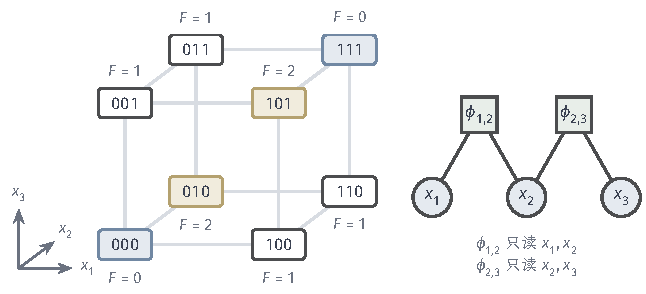
\includegraphics[width=109.269mm]{figures/01-basic-mathematics/04-graphs/tikz/c5-configuration-scopes/figure.pdf}
  \caption{配置空间与局部作用域。左：三个二值变量的$8$种配置排在立方体的顶点上，顶点旁的数是总成本$F=\phi_{1,2}+\phi_{2,3}$，其中相邻变量取值不同时成本为$1$；蓝色顶点成本为$0$，黄色顶点成本为$2$。右：圆点表示变量，方块表示局部函数，连线表示该函数读取的变量。每个局部函数只读取两个变量，但它们的和仍然对全部$8$种配置给出成本。}
  \label{fig:graph-dp-configuration-scopes}
\end{figure}

把这个例子一般化。设有一组局部项，用下标$a\in A$区分，每一项$\phi_a$只读取下标集合$S_a\subseteq V$中的变量，总成本为
\begin{equation}
F(\bm x)=\sum_{a\in A}\phi_a(\bm x_{S_a}),\qquad \bm x\in\mathcal X .
\label{eq:graph-dp-local-sum}
\end{equation}
这里的$\phi_a$称为\term{局部函数}（local function），也常称为\term{因子}（factor）；它读取的下标集合$S_a$称为$\phi_a$的\term{作用域}（scope）。

“局部”限定的是读取范围，不是精度：$\phi_a$精确地给出$\bm x_{S_a}$每种取值的成本，并不是对某个整体函数的近似。作用域也不限于两个变量，三元、四元的局部函数同样允许；一元项$\phi_i(x_i)$是作用域为$\{i\}$的特例，作用域为空集的项是一个常数。

局部函数的取值允许为$+\infty$，用来表示禁止的组合。例如设备$1,2$不能同时打开时，可以令$\phi_{1,2}(1,1)=+\infty$。本部分固定如下运算约定：$+\infty$加任何有限数或$+\infty$仍得$+\infty$；比较大小时$+\infty$大于每个实数，因而有限集合中只要有一个有限数，最小值就是有限的。这样，只要某一项禁止，整个配置的总成本就是$+\infty$。

总成本有限的配置称为\term{可行配置}。同一个式~\eqref{eq:graph-dp-local-sum}因此既表达偏好，也表达约束。若最小值为$+\infty$，说明每个配置都被某项禁止，所以求最小值同时回答了是否存在可行配置。

式~\eqref{eq:graph-dp-local-sum}的分解由问题给出，不是自动成立的性质。任意函数$F$都可以写成作用域为$V$的单个“局部”函数，但这时局部函数表就有$|\mathcal X|$项，与直接枚举没有区别。本部分始终假定分解已经给定，并且各作用域都较小；从一个任意给定的整体函数中寻找小作用域分解，是另一个问题。

\subsection{依赖图与因子图}
\label{sec:graph-dp-factor-graphs}

要利用“某一项不读某个变量”，首先要知道哪些变量出现在同一个局部函数里。这是一种纯粹的结构信息，可以用几种图来记录，它们保留和丢失的内容各不相同。

只有成对局部项时，可以以变量为顶点，两个变量出现在同一个成对项中就连一条边。三台设备的例子得到路径$1-2-3$。这样的图记录的是函数的依赖关系，不是变量的取值本身；称“依赖结构是一条链”或“是一棵树”，指的就是这个依赖图是路径或树。

三元及更高阶的局部项无法用一条边表示。这时把变量和局部函数分成两类节点：每个变量一个圆形节点，每个局部函数一个方形节点；变量属于某个局部函数的作用域时，在两者之间连边。这样得到的二部图称为\term{因子图}（factor graph）。因子图保留了每个局部函数的身份：两个不同的局部函数即使作用域相同，也是两个不同的方形节点。图~\ref{fig:graph-dp-configuration-scopes}右侧就是三台设备例子的因子图。

\paragraph{原始图与超图}
看一个含三元项的例子，后文称为\emph{三元作用域例子}：四个二值变量$x_1,\ldots,x_4$，两个局部函数$\phi_A(x_1,x_2,x_3)$与$\phi_B(x_2,x_3,x_4)$，作用域为$S_A=\{1,2,3\}$和$S_B=\{2,3,4\}$。它们的数值在下一小节给出，这里只看结构。

除因子图外，还有两种常用的结构表示。第一种不保留函数节点，把每个作用域内的变量两两连边，得到的图称为\term{原始关系图}（primal graph），简称原始图。这里原始图有边$\{1,2\},\allowbreak\{1,3\},\allowbreak\{2,3\},\allowbreak\{2,4\},\allowbreak\{3,4\}$，唯独缺少$\{1,4\}$，因为变量$1$和$4$从不出现在同一个局部函数中。每个作用域在原始图中都是两两相邻的顶点组。

第二种允许一条“边”包含任意多个顶点：每个作用域记为一条\term{超边}（hyperedge），由此得到\term{超图}（hypergraph）。这里超图有两条超边$\{1,2,3\}$和$\{2,3,4\}$。图~\ref{fig:graph-dp-three-representations}并排画出了三种表示。

\begin{figure}[!htb]
  \centering
  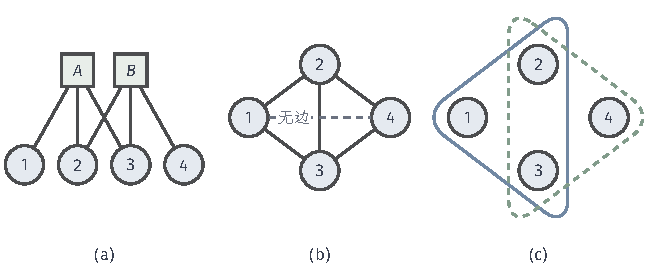
\includegraphics[width=111.936mm]{figures/01-basic-mathematics/04-graphs/tikz/c5-three-representations/figure.pdf}
  \caption{作用域$\{1,2,3\}$与$\{2,3,4\}$的三种结构表示。左：因子图，方块$A$、$B$是两个局部函数，连线表示读取关系。中：原始关系图，把每个作用域内的变量两两相连，只缺边$\{1,4\}$。右：超图，蓝色实线与绿色虚线围出的区域各是一条超边。若把两个三元函数换成五条边上的五个成对函数，原始图完全相同，而因子图和超图都会改变。}
  \label{fig:graph-dp-three-representations}
\end{figure}

\paragraph{原始图丢失的信息}
原始图丢失了作用域的分组：若把$\phi_A,\phi_B$换成定义在五条边上的五个成对局部函数，原始图不变，因子图和超图却不同。

更重要的是，相同的两两连接不能恢复函数表。设另有两个作用域同为$\{1,2,3\}$与$\{2,3,4\}$的局部函数：$\chi_A(x_1,x_2,x_3)$在$x_1+x_2+x_3$为偶数时取$0$、为奇数时取$+\infty$，$\chi_B$对$x_2+x_3+x_4$作同样的规定。$\chi_A$允许的取值恰为$(0,0,0),(0,1,1),(1,0,1),(1,1,0)$，其中任意两个变量的四种取值组合都出现过。

因此，若只保留“每对变量允许哪些取值”的成对规则，这些规则什么也不禁止，$16$种配置都会被放行。而原问题中$x_2,x_3$确定后，$x_1$和$x_4$都被奇偶条件唯一确定，只有$4$种可行配置。三元规则不是成对规则的叠加。

超图保住了作用域的分组，但和原始图一样不保存局部函数的数值；因子图保住了函数身份，也仍需另外存储每个函数的取值表。第~\ref{chap:general-graph-dp-construction}章构建计算结构时以原始图为依据，因为原始图上的边已经足以说明哪些变量必须同时出现，并且每个作用域都能整体放进构建出的某个计算单元（第~\ref{sec:graph-dp-clique-containment}小节）。计算时则始终使用完整的局部函数，不把它们拆成成对规则。

\subsection{计算任务与输出}
\label{sec:graph-dp-problem}

本部分的输入由两部分组成：每个变量的有限状态集合$\mathcal X_i$；一组局部函数$\phi_a$，每个以作用域$S_a$和一张取值表给出。取值表对$\bm x_{S_a}$的每种取值列出一个属于$\mathbb R\cup\{+\infty\}$的数，共$\prod_{i\in S_a}|\mathcal X_i|$项。在这同一份输入上，可以提出几种不同的计算任务。

最基本的任务是最小成本：
\begin{enumerate}
  \item 求最小成本$F^\star=\min_{\bm x\in\mathcal X}F(\bm x)$；
  \item 若$F^\star<+\infty$，给出一个最优配置$\bm x^\star$，即满足$F(\bm x^\star)=F^\star$的配置；若$F^\star=+\infty$，报告不存在可行配置。
\end{enumerate}

有时不想把全部变量都优化掉，而要保留一组变量$R\subseteq V$，对它们的每种取值给出其余变量取最优时的成本，即一张以$\bm x_R$为索引的表
\[
F_R(\bm x_R)=\min_{\bm x_{V\setminus R}}F(\bm x_R,\bm x_{V\setminus R}).
\]
这张表回答“若把这几个变量固定成某组值，最好能做到多少”。它的输出本身有$\prod_{i\in R}|\mathcal X_i|$项，$R=\varnothing$时退化为单个数$F^\star$。

另外两种任务不再挑选一个配置，而是对全部配置汇总。第一种是计数：可行配置有多少个。第二种是加权求和：给每个局部函数一张非负权重表，把配置的权重定义为各局部权重之积，求全部配置的权重总和。这两种任务的组合方式（相乘）和汇总方式（求和）都与最小成本不同，第~\ref{sec:graph-dp-semiring}节统一展开。

\paragraph{三元作用域例子的数值}
三元作用域例子的总成本为$F=\phi_A+\phi_B$，两张表由表~\ref{tab:graph-dp-ternary-tables}给出，其中$+\infty$表示禁止的组合。

\begin{table}[!htb]
  \centering
  \begin{tabular}{ccccccccc}
    \toprule
    取值 & $000$ & $001$ & $010$ & $011$ & $100$ & $101$ & $110$ & $111$\\
    \midrule
    $\phi_A(x_1,x_2,x_3)$ & $1$ & $0$ & $2$ & $+\infty$ & $0$ & $2$ & $1$ & $2$\\
    $\phi_B(x_2,x_3,x_4)$ & $2$ & $1$ & $0$ & $+\infty$ & $+\infty$ & $0$ & $1$ & $2$\\
    \bottomrule
  \end{tabular}
  \caption{三元作用域例子的两个局部函数。第一列的三位二进制串对$\phi_A$表示$(x_1,x_2,x_3)$，对$\phi_B$表示$(x_2,x_3,x_4)$。}
  \label{tab:graph-dp-ternary-tables}
\end{table}

最直接的做法是按字典序逐个检查全部配置，保留目前最小的成本$\hat F$（初始为$+\infty$）及其配置，遇到更小的成本就替换，全部检查完后停止。在这个例子上，枚举$16$个配置得$F^\star=0$，唯一的最优配置为$\bm x^\star=(0,0,1,0)$，可行配置共$10$个；后面用这一例子演示消元时，都用这一结果核对。

枚举总是正确，但要读$|\mathcal X|\cdot|A|$次表，各变量至多$q$个状态时可达$|A|\,q^n$。它把每个配置当作整体，没有利用“某一项不读某个变量”这一信息。下一节从链和树开始利用这一信息。

% 第11章第2节：链与树上的接口递推（固定接口后的子问题、链上的递推与回溯、树上的消息递推）。

\section{链与树上的接口递推}
\label{sec:graph-tree-dp}

依赖图没有环、局部项至多读取两个变量时，可以把变量分成只通过一个变量相连的两侧。本节先在小例子上看清“固定这个变量、分别处理两侧”为什么可行，以及要保留什么；再把这一动作在链上从一端推到另一端，在树上从叶推到根，每一步的接口都是单个变量。带环的情形留到下一节。

\subsection{固定接口后的子问题}
\label{sec:graph-dp-tree-idea}

\paragraph{接口变量}
回到第~\ref{sec:graph-dp-scopes}小节的三台设备。若先把$x_2$固定为某个值，$\phi_{1,2}$只剩$x_1$可变，$\phi_{2,3}$只剩$x_3$可变，两项不再共享任何变量，于是$x_1$和$x_3$可以分别选择：
\[
\min_{x_1,x_2,x_3}F=\min_{x_2}\Bigl[\min_{x_1}\phi_{1,2}(x_1,x_2)+\min_{x_3}\phi_{2,3}(x_2,x_3)\Bigr].
\]
对$x_2$的每个取值，两个内层最小值各只比较两个数。

这里$x_2$起着\term{接口}（interface）的作用：它把其余变量分成两侧，一侧的选择只通过$x_2$影响另一侧。好比两个房间之间只有一扇门，只要知道门开着还是关着，每个房间里怎样安排最好就可以各自决定。于是对接口的每种取值，先把一侧最好的成本算出来，记成一张以接口取值为索引的表，另一侧只需查表。

本部分反复使用的就是这个动作：固定一组接口变量，把只在一侧出现的变量汇总掉，留下一张以接口取值为索引的表。链和树上，接口可以沿依赖结构依次找到；一般依赖结构上接口要包含多个变量，怎样找到它们是第~\ref{chap:general-graph-dp-construction}章的问题。

\paragraph{成对成本的模型}
本节只考虑一元项和成对项，并假定成对项组成的依赖图没有环。这时总成本为
\begin{equation}
F(\bm x)=\sum_{i\in V}\phi_i(x_i)+\sum_{\{u,v\}\in E}\phi_{u,v}(x_u,x_v),
\label{eq:graph-dp-pairwise-cost}
\end{equation}
其中$\mathcal G=(V,E)$是依赖图，$\phi_{u,v}(x_u,x_v)$与$\phi_{v,u}(x_v,x_u)$指同一个局部函数。没有一元项的变量可以取$\phi_i\equiv0$。输入是各变量的状态集合、一元项表和每条边上的成对项表；输出是最小成本$F^\star$和一个最优配置，$F^\star=+\infty$时报告不可行。

\paragraph{三变量链}
先看三个变量的链$1-2-3$，每个变量取三档$\{0,1,2\}$，总成本$F=\phi_{1,2}(x_1,x_2)+\phi_{2,3}(x_2,x_3)$。两张局部函数表按行列给出：
\[
\bigl[\phi_{1,2}(x_1,x_2)\bigr]=\begin{bmatrix}4&1&3\\2&3&5\\3&4&2\end{bmatrix},\qquad
\bigl[\phi_{2,3}(x_2,x_3)\bigr]=\begin{bmatrix}1&3&2\\4&3&5\\2&2&4\end{bmatrix},
\]
左表的行对应$x_1=0,1,2$、列对应$x_2=0,1,2$，右表的行对应$x_2$、列对应$x_3$。直接枚举要计算$3^3=27$个配置的成本。

$x_1$只出现在$\phi_{1,2}$中。若先把$x_2$固定为某个值，$x_1$的选择就不再影响$\phi_{2,3}$，只需在左表的这一列中取最小。对$x_2=0,1,2$分别取列最小值，得到一张只依赖$x_2$的表
\[
m_{1\to2}(x_2)=\min_{x_1}\phi_{1,2}(x_1,x_2)=(2,\,1,\,2),
\]
达到最小值的$x_1$依次为$1,0,2$。这张表概括了链左端的全部信息：无论右侧怎样取值，只要$x_2$给定，左端最好的做法和它的成本都已确定。

剩下只需在$x_2,x_3$上求
\[
\min_{x_2,x_3}\bigl[m_{1\to2}(x_2)+\phi_{2,3}(x_2,x_3)\bigr].
\]
对$x_2=0,1,2$，括号内对$x_3$的最小值依次为
\[
2+1=3,\qquad 1+3=4,\qquad 2+2=4,
\]
所以最优成本为$3$，在$x_2=0,x_3=0$时达到，再查表得$x_1=1$。

整个过程计算了$9+9=18$个候选值，而不是$27$个配置；链越长，节省越多。

\paragraph{为什么要保留整张表}
左端交给右侧的必须是一张以接口取值为索引的表，而不只是左端的一个最优值。左表的最小值是$1$，在$(x_1,x_2)=(0,1)$处达到；若左端只报告“我最少付$1$，此时$x_2=1$”，右侧只能在$x_2=1$下选$x_3$，得到
\[
1+\min(4,3,5)=4.
\]
而整体最优配置$(1,0,0)$中左端付的是$\phi_{1,2}(1,0)=2$，比左端自己的最优值大，却让右端只付$1$。

左端事先无法知道右端偏好哪个$x_2$，所以要对接口的每个取值都给出条件最小成本，把选择$x_2$的决定留到两侧的成本都已知之后。

图~\ref{fig:graph-dp-interface-options}将左右两侧的条件最小值按$x_2$对齐。左侧最便宜的是中列，合并后最便宜的却是左列；保留整张表，才能把这一选择留给整体成本。

\begin{figure}[!htb]
  \centering
  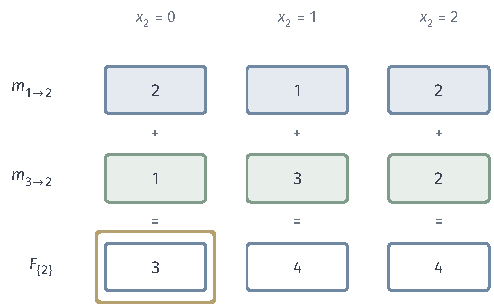
\includegraphics[width=83.608mm]{figures/03-graphs/04-local-functions-and-dynamic-programming/tikz/dp-interface-options/figure.pdf}
  \caption{接口表保留选择余地。沿用三档链的两张成本表，上排是对$x_1$取最小得到的$(2,1,2)$，中排是对$x_3$取最小得到的$(1,3,2)$，下排按同一$x_2$逐列相加。黄色边框标出整体最优值$3$所在的$x_2=0$，它并不对应上排的最小值。}
  \label{fig:graph-dp-interface-options}
\end{figure}

\paragraph{最小值的三条规则}
这样分步的依据是有限集合上最小值的三条规则。设$y,z$分别在有限集合中取值，$h$、$g$取值于$\mathbb R\cup\{+\infty\}$，$c$与$y$无关，则
\begin{equation}
\min_{y,z}h(y,z)=\min_{z}\min_{y}h(y,z),\qquad
\min_{y}\bigl[g(y)+c\bigr]=\min_{y}g(y)+c,
\label{eq:graph-dp-min-rules}
\end{equation}
并且对取值于互不相交变量组$y_1,\ldots,y_k$的函数，
\[
\min_{y_1,\ldots,y_k}\sum_{r}g_r(y_r)=\sum_r\min_{y_r}g_r(y_r).
\]

第一条成立，因为两边都是同一个有限数集中的最小元。第二条成立，因为加上同一个$c$不改变比较结果。第三条成立，因为各$y_r$可以分别取到各自的最小点，而任何选择都不会使某一项小于它的最小值。$c$或某项为$+\infty$时，按第~\ref{sec:graph-dp-scopes}小节的运算约定，三条规则依然成立。

在三变量链上，$\phi_{2,3}$对$x_1$而言是固定加项，由第一、二条，$\min_{x_1}$可以移到$\phi_{1,2}$上。

\subsection{链上的递推与回溯}
\label{sec:graph-dp-chain}

\subsubsection{问题与思路}

现在设链为$1-2-\cdots-n$，总成本含一元项$\phi_k(x_k)$和相邻成对项$\phi_{k-1,k}(x_{k-1},x_k)$。三变量链上的汇总可以从左端开始一步一步向右推进，每一步把接口右移一个变量。

推进到第$k$个变量时，左边的$x_1,\ldots,x_{k-1}$已经汇总掉，留下一张以$x_k$为索引的表$D_k(x_k)$：$x_k$取某个状态时，前$k$个变量的局部项
\[
\sum_{i=1}^{k}\phi_i(x_i)+\sum_{i=2}^{k}\phi_{i-1,i}(x_{i-1},x_i)
\]
对$x_1,\ldots,x_{k-1}$求最小值的结果，称为前$k$个变量的最小部分成本。这里$x_k$是已处理部分与其余部分之间的接口，$D_k$就是上一小节所说的条件最小成本表。

只有第一个变量时没有需要汇总的变量，$D_1(x_1)=\phi_1(x_1)$。从$D_{k-1}$得到$D_k$只需再汇总一个变量$x_{k-1}$：对$x_k$的每个状态，把前$k-1$个变量的最小部分成本加上连接两者的成对项，对$x_{k-1}$取最小值，再加上$x_k$自己的一元项，即
\begin{equation}
\begin{gathered}
D_1(x_1)=\phi_1(x_1),\\
D_k(x_k)=\phi_k(x_k)+\min_{x_{k-1}\in\mathcal X_{k-1}}\bigl[D_{k-1}(x_{k-1})+\phi_{k-1,k}(x_{k-1},x_k)\bigr],\quad k=2,\ldots,n.
\end{gathered}
\label{eq:graph-dp-chain-recursion}
\end{equation}
整条链的最小成本是
\[
F^\star=\min_{x_n}D_n(x_n).
\]
这种把问题按顺序拆开、为每个子问题保存最优值表并由前一张表算出后一张表的做法称为\term{动态规划}（dynamic programming）。

最小值只告诉我们最小成本是多少，不直接给出达到它的配置。取最小值时，“是哪一个$x_{k-1}$达到最小”被丢掉了；若只保存$D_k$，事后只能重新枚举。所以每算一个$D_k(x_k)$，都顺手记下达到最小值的$x_{k-1}$，组成\term{回溯表}$p_k(x_k)$。

算完以后从末端出发：$x_n$取使$D_n$最小的状态，再由$p_n(x_n)$读出$x_{k-1}$，逐个向左读到$x_1$。并列最优时需要事先固定选择规则，本节约定取编号最小的状态。

\subsubsection{算法实现}

链的次序、各变量的状态集合和局部函数表都由输入给定，运行中不变。算法维护三项状态：
\begin{itemize}
  \item 最小部分成本表$D_k$，$k=1,\ldots,n$：每张以$x_k$为索引，至多$q$项；初始只有$D_1=\phi_1$；
  \item 回溯表$p_k$，$k=2,\ldots,n$：$p_k(x_k)$是达到$D_k(x_k)$时$x_{k-1}$的取值；初始为空；
  \item 轮次$k$：已经算出的最后一张表的下标，初值为$1$。
\end{itemize}
此后每一轮令$k\gets k+1$，对$x_k$的每个状态$s$做两件事：
\begin{itemize}
  \item 列候选：对$x_{k-1}$的每个状态$r$，计算$D_{k-1}(r)+\phi_{k-1,k}(r,s)$，即式~\eqref{eq:graph-dp-chain-recursion}方括号中的值；
  \item 取最小：令$D_k(s)$等于一元项$\phi_k(s)$加上最小的候选值，$p_k(s)$为达到它的$r$，并列时取编号最小者。
\end{itemize}
第$n$轮之后递推停止。若$\min_{x_n}D_n(x_n)=+\infty$，报告不可行；否则按下面两步恢复配置：
\begin{itemize}
  \item 定末端：$x_n$取使$D_n$最小的状态，并列取编号最小者；
  \item 逆向读取：对$k=n,\ldots,2$，令$x_{k-1}=p_k(x_k)$。
\end{itemize}

\begin{algorithm}[链上的最小成本递推]
\label{alg:graph-dp-chain}
输入：链上各变量的有限状态集合、一元项表和相邻成对项表。输出：最小成本和一个最优配置。
\begin{enumerate}
  \item 令$D_1(x_1)=\phi_1(x_1)$。
  \item 对$k=2,\ldots,n$和每个$x_k$，计算式~\eqref{eq:graph-dp-chain-recursion}方括号中的全部候选值，取最小值记为$D_k(x_k)$，并把达到最小值的$x_{k-1}$（并列时取编号最小者）记为$p_k(x_k)$。
  \item 若$\min_{x_n}D_n(x_n)=+\infty$，报告不可行并停止。否则取使$D_n$最小的$x_n$（并列取编号最小者）；再对$k=n,\ldots,2$令$x_{k-1}=p_k(x_k)$。
\end{enumerate}
\end{algorithm}

\paragraph{执行过程}
取$n=4$的二值链，一元项为$\phi_1=(0,3)$、$\phi_2=(2,0)$、$\phi_3=(3,0)$、$\phi_4=(1,2)$，括号内依次是取$0$和取$1$的成本；相邻成对项在两端取值相同时为$0$，不同时为$2$。表~\ref{tab:graph-dp-chain-trace}列出各轮的候选与结果，逐轮看：
\begin{itemize}
  \item 第$1$轮：$D_1=\phi_1=(0,3)$。
  \item 第$2$轮：$x_2=0$的候选为$D_1(0)+0=0$与$D_1(1)+2=5$，加一元项$2$得$D_2(0)=2$；$x_2=1$的候选为$D_1(0)+2=2$与$D_1(1)+0=3$，加一元项$0$得$D_2(1)=2$。两处都由$x_1=0$达到，$p_2=(0,0)$。
  \item 第$3$轮：$x_3=0$的候选为$2,4$，加$3$得$5$；$x_3=1$的候选为$4,2$，加$0$得$2$。$D_3=(5,2)$，$p_3=(0,1)$。
  \item 第$4$轮：$x_4=0$的候选为$5,4$，加$1$得$5$；$x_4=1$的候选为$7,2$，加$2$得$4$。$D_4=(5,4)$，$p_4=(1,1)$。
\end{itemize}
第$4$轮后停止。$\min D_4=\min(5,4)=4$，在$x_4=1$处达到。沿回溯表逆向读取：
\[
x_3=p_4(1)=1,\qquad x_2=p_3(1)=1,\qquad x_1=p_2(1)=0,
\]
得到最优配置$(0,1,1,1)$。图~\ref{fig:graph-dp-chain-recursion}把同一过程画成每一轮的表和每个状态选中的前驱。

\begin{table}[!htb]
  \centering
  \small
  \begin{tabular}{@{}cccccccc@{}}
    \toprule
    & & \multicolumn{3}{c}{$x_k=0$} & \multicolumn{3}{c}{$x_k=1$}\\
    \cmidrule(lr){3-5}\cmidrule(lr){6-8}
    $k$ & $\phi_k$ & 候选 & $D_k(0)$ & $p_k(0)$ & 候选 & $D_k(1)$ & $p_k(1)$\\
    \midrule
    $1$ & $(0,3)$ & — & $0$ & — & — & $3$ & —\\
    $2$ & $(2,0)$ & $0,\ 5$ & $2$ & $0$ & $2,\ 3$ & $2$ & $0$\\
    $3$ & $(3,0)$ & $2,\ 4$ & $5$ & $0$ & $4,\ 2$ & $2$ & $1$\\
    $4$ & $(1,2)$ & $5,\ 4$ & $5$ & $1$ & $7,\ 2$ & $4$ & $1$\\
    \bottomrule
  \end{tabular}
  \caption{四变量二值链上的逐轮计算。“候选”一栏是式~\eqref{eq:graph-dp-chain-recursion}方括号中对$x_{k-1}=0,1$的两个值；$D_k$等于一元项加上候选中的较小者，$p_k$是达到较小者的$x_{k-1}$。}
  \label{tab:graph-dp-chain-trace}
\end{table}

\begin{figure}[!htb]
  \centering
  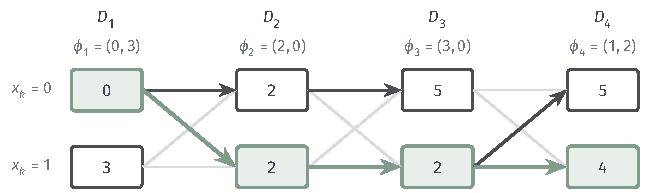
\includegraphics[width=109.587mm]{figures/01-basic-mathematics/04-graphs/tikz/c5-chain-recursion/figure.pdf}
  \caption{四变量二值链上的递推表。每列是一个变量，上下两格分别是$D_k(0)$与$D_k(1)$，列上方的小字为一元项。两列之间的灰色线表示全部候选，箭头从每个状态选中的前驱指向该状态，即回溯表$p_k$记录的选择。末列中$D_4(1)=4$最小，沿绿色箭头逆向读取得到最优配置$(0,1,1,1)$。逐点选取一元项最小的状态会得到$(0,1,1,0)$，成本为$5$。}
  \label{fig:graph-dp-chain-recursion}
\end{figure}

\subsubsection{算法分析}

\paragraph{正确性}
递推的正确性在于每张表$D_k$确实是前$k$个变量的最小部分成本。对$k$归纳。

$k=1$时没有被汇总的变量，结论就是定义。设结论对$k-1$成立。前$k$个变量的部分成本等于前$k-1$个变量的部分成本加上$\phi_{k-1,k}(x_{k-1},x_k)+\phi_k(x_k)$，后两项不含$x_1,\ldots,x_{k-2}$。按式~\eqref{eq:graph-dp-min-rules}的第一条，对$x_1,\ldots,x_{k-1}$求最小值可以先对$x_1,\ldots,x_{k-2}$、再对$x_{k-1}$进行；按第二条，先求的那一步可以越过后两项，只作用在前$k-1$个变量的部分成本上，由归纳假设得到$D_{k-1}(x_{k-1})$。

再对$x_{k-1}$求最小值，并把与$x_{k-1}$无关的$\phi_k(x_k)$移出，就得到式~\eqref{eq:graph-dp-chain-recursion}。取$k=n$，前$n$个变量的部分成本就是$F$，所以
\[
\min_{x_n}D_n(x_n)=F^\star.
\]

回溯得到的配置达到这个最小值。从末端起逐步向左，每一步选的$x_{k-1}=p_k(x_k)$都达到式~\eqref{eq:graph-dp-chain-recursion}中的最小值，于是读出的$x_1,\ldots,x_k$使前$k$个变量的部分成本恰好等于$D_k(x_k)$；读到$x_1$时，整个配置的成本等于$D_n(x_n)=F^\star$。这一论证要求$F^\star$有限；$F^\star=+\infty$时每个配置都“达到”最小值，所以算法报告不可行，而不输出配置。

\paragraph{与逐点选择的比较}
成对项正是逐点选择失效的原因。让每个变量只看自己的一元项、各自取最小，在上面的二值链中会选$(0,1,1,0)$：一元项合计为$1$，但两处取值变化要付$4$，总成本为$5$。递推得到的$(0,1,1,1)$在$x_4$上多付了$1$个单位的一元成本，却省掉了最后一处变化，总成本为$4$。$D_k$之所以能避免这种短视，是因为它对$x_k$的每个状态都保留了“左侧最好能做到多少”，等后面的变量看过成对项以后再决定$x_k$取哪个状态。

\paragraph{复杂度}
设每个变量至多有$q$个状态。每一轮为$x_k$的每个状态比较至多$q$个候选，共至多$q^2$次候选计算，整条链约$nq^2$次；$D_k$与$p_k$各至多$q$项，共约$2nq$项。若只要最优值而不恢复配置，任一时刻只需保留上一轮的表。与$q^n$个配置的枚举相比，开销从指数降为线性于$n$。

\subsection{树上的消息递推}
\label{sec:graph-dp-tree-messages}

\subsubsection{问题与思路}

树没有链那样的天然顺序，但选定一个根$\rho$以后，每个非根顶点都有唯一的父点（第~\ref{sec:graph-trees-forests}节）。链上的$D_{k-1}$概括了$x_k$左侧的全部变量；树上一个顶点可能有多个子点，每个子点下面挂着一棵子树，需要分别概括后再合并。

对树的一条边$\{u,v\}$，删去它以后树分成两部分，记含$u$的那部分顶点集为$V_{u|v}$，称为$u$一侧。$u$一侧的变量只通过这条边与其余部分发生联系，$x_v$就是这一侧与其余部分之间的接口：只要$x_v$给定，$u$一侧的变量最好怎样取值、最少要付多少成本就确定了。

把这个“最少要付多少”对$x_v$的每个状态列出来，就得到一张报价单：“你取$0$，我这边最少付多少；你取$1$，最少付多少”。$v$拿到报价单，不必知道$u$一侧有哪些变量、怎样取值，就能在决定自己的状态时把那一侧的成本算进去。

以图~\ref{fig:graph-dp-message-side}的五顶点树为例，删去边$\{3,4\}$后，$4$一侧是$\{4,5\}$。$x_3=0$时，这一侧最便宜的取法是$(x_4,x_5)=(0,1)$：一元项$\phi_4(0)+\phi_5(1)=0$，边$\{3,4\}$两端相同不付费，边$\{4,5\}$两端不同付$1$，合计$1$。

$x_3=1$时最便宜的是$(1,1)$，只付一元项$\phi_4(1)=1$。于是$4$向$3$报出的价目是$(1,1)$。

\begin{figure}[!htb]
  \centering
  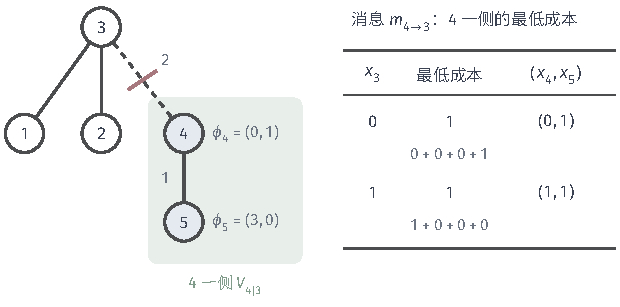
\includegraphics[width=104.902mm]{figures/01-basic-mathematics/04-graphs/tikz/c5-message-side/figure.pdf}
  \caption{消息是一侧的报价单。左：删去边$\{3,4\}$（虚线，旁边的$2$是两端取值不同时的成本），绿色区域是$4$一侧$V_{4|3}=\{4,5\}$，边$\{4,5\}$两端不同时成本为$1$。右：$x_3$取各状态时，$4$一侧的最低成本及达到它的取值；小字依次是$\phi_4$、$\phi_5$、边$\{3,4\}$、边$\{4,5\}$的成本。回溯表$b_{4\to3}$只记录其中$x_4$的取值$(0,1)$，$x_5$由$b_{5\to4}$给出。}
  \label{fig:graph-dp-message-side}
\end{figure}

这张报价单称为从$u$发往$v$的\term{消息}（message）。它可以逐层算出：$u$一侧除$u$本身以外，按$u$的其他邻居$r$分成几块，每块的最低成本已由消息$m_{r\to u}$报给$u$；$u$把自己的一元项、各块报来的价目和边$\{u,v\}$上的成对项相加，再替自己选最好的状态，即
\begin{equation}
\begin{aligned}
m_{u\to v}(x_v)=\min_{x_u\in\mathcal X_u}\Bigl[&\phi_u(x_u)+\phi_{u,v}(x_u,x_v)\\
&+\sum_{r\in N(u)\setminus\{v\}}m_{r\to u}(x_u)\Bigr],
\end{aligned}
\label{eq:graph-dp-tree-message}
\end{equation}
其中$N(u)$是$u$在依赖图中的邻居集合。消息等于$u$一侧在$x_v$固定时的最低成本，这一含义在第~\ref{sec:graph-dp-tree-analysis}小节证明。叶顶点只有一个邻居，求和为空，消息只由它自己的一元项和边上的成对项算出。链上的$D_k(x_k)$正是$\phi_k(x_k)+m_{k-1\to k}(x_k)$。

式~\eqref{eq:graph-dp-tree-message}右端用到$u$的其他邻居发来的消息，所以要从叶开始算，每个顶点等全部子点报完价再向父点报价；全部报到根以后，根把一元项与各条入消息相加，就得到整棵树在根取各状态时的最低成本。

与链上一样，取最小值丢掉了达到者，所以算每条消息时同时为接收端的每个状态$x_v$记下达到最小值的$x_u$，组成回溯表$b_{u\to v}(x_v)$。根选定状态以后，每个子点只需按父点的取值查自己的回溯表，就能沿树向外恢复整个配置。

\subsubsection{算法实现}

计算开始前任选根$\rho$，求出每个顶点的父点$p(u)$和一个后序，即先列出全部子点、再列出父点的顶点序列，可由一次深度优先遍历的完成次序得到。根、父点和后序只规定计算次序，运行中不变，与局部函数表一样不算状态。算法维护四项状态：
\begin{itemize}
  \item 消息表$m_{u\to p(u)}$，每个非根顶点$u$一张，以父点的取值$x_{p(u)}$为索引；初始均未计算；
  \item 回溯表$b_{u\to p(u)}$，与消息表一一对应，记录达到最小值的$x_u$；初始为空；
  \item 根处的合并值$g_\rho(x_\rho)$：根取各状态时整棵树的最低成本；向上一遍结束后才算出；
  \item 配置$\bm x$：初始各变量均未赋值，回溯时逐个写入。
\end{itemize}
向上一遍按后序依次处理非根顶点$u$，记$v=p(u)$。此时$u$的全部子点都已处理，消息$m_{r\to u}$都已算出。每处理一个顶点做三件事：
\begin{itemize}
  \item 汇总入消息：对$x_u$的每个状态，计算$\phi_u(x_u)+\sum_{r\in N(u)\setminus\{v\}}m_{r\to u}(x_u)$，即$u$及其子树在$x_u$固定时的最低成本；
  \item 列候选：对$x_v$的每个状态和$x_u$的每个状态，在上一步的值上加$\phi_{u,v}(x_u,x_v)$，得到式~\eqref{eq:graph-dp-tree-message}方括号中的值；
  \item 取最小：对$x_v$的每个状态，把最小的候选值记为$m_{u\to v}(x_v)$，达到它的$x_u$（并列取编号最小者）记为$b_{u\to v}(x_v)$。
\end{itemize}
全部非根顶点处理完后，在根处合并：
\[
g_\rho(x_\rho)=\phi_\rho(x_\rho)+\sum_{r\in N(\rho)}m_{r\to\rho}(x_\rho),
\]
最小成本为$\min_{x_\rho}g_\rho(x_\rho)$。若它为$+\infty$，报告不可行并停止；否则向外一遍恢复配置：
\begin{itemize}
  \item 定根：$x_\rho$取使$g_\rho$最小的状态，并列取编号最小者；
  \item 查表：按前序（后序的逆序，父点总在子点之前）处理非根顶点$u$，令$x_u=b_{u\to p(u)}(x_{p(u)})$。轮到$u$时父点已经赋值，所以查表总能进行。
\end{itemize}
每个非根顶点恰好赋值一次，全部变量赋值后停止。

\begin{algorithm}[树上的消息递推]
\label{alg:graph-dp-tree-messages}
输入：依赖树上各变量的有限状态集合、一元项表和各边的成对项表。输出：最小成本和一个最优配置，或不可行报告。
\begin{enumerate}
  \item 任选根$\rho$，求出父点$p(u)$与一个后序。
  \item 按后序处理每个非根顶点$u$，记$v=p(u)$：对$x_v$的每个状态，枚举$x_u$的全部状态，按式~\eqref{eq:graph-dp-tree-message}计算候选值，取最小者记为$m_{u\to v}(x_v)$，达到它的$x_u$（并列取编号最小者）记为$b_{u\to v}(x_v)$。
  \item 计算$g_\rho(x_\rho)=\phi_\rho(x_\rho)+\sum_{r\in N(\rho)}m_{r\to\rho}(x_\rho)$。若$\min_{x_\rho}g_\rho(x_\rho)=+\infty$，报告不可行并停止。
  \item 取使$g_\rho$最小的$x_\rho$（并列取编号最小者）；按前序对每个非根顶点$u$令$x_u=b_{u\to p(u)}(x_{p(u)})$。
\end{enumerate}
\end{algorithm}

\paragraph{执行过程}
沿用图~\ref{fig:graph-dp-message-side}的树：边为$\{1,3\},\allowbreak\{2,3\},\allowbreak\{3,4\},\allowbreak\{4,5\}$，以$3$为根；二值一元项为$\phi_1=(0,2)$、$\phi_2=(2,0)$、$\phi_3=(1,0)$、$\phi_4=(0,1)$、$\phi_5=(3,0)$；成对项在两端相同时为$0$，不同时分别为$1,1,2,1$（按上面边的顺序）。父点为$p(1)=p(2)=p(4)=3$、$p(5)=4$，取后序$1,2,5,4,3$。向上一遍依次处理四个非根顶点，表~\ref{tab:graph-dp-tree-trace}列出每条消息的候选：
\begin{itemize}
  \item 处理$1$：叶顶点，汇总值就是$\phi_1=(0,2)$。$x_3=0$的候选为$0+0$与$2+1$，$x_3=1$的候选为$0+1$与$2+0$，得$m_{1\to3}=(0,1)$，两处都由$x_1=0$达到，$b_{1\to3}=(0,0)$。
  \item 处理$2$：汇总值为$\phi_2=(2,0)$，得$m_{2\to3}=(1,0)$，$b_{2\to3}=(1,1)$：无论$x_3$取什么，$x_2$都取$1$更便宜。
  \item 处理$5$：汇总值为$\phi_5=(3,0)$，得$m_{5\to4}=(1,0)$，$b_{5\to4}=(1,1)$。
  \item 处理$4$：子点$5$的消息已经算出，汇总值为$\phi_4+m_{5\to4}=(0+1,\ 1+0)=(1,1)$。$x_3=0$的候选为$1+0$与$1+2$，$x_3=1$的候选为$1+2$与$1+0$，得$m_{4\to3}=(1,1)$，$b_{4\to3}=(0,1)$，与图~\ref{fig:graph-dp-message-side}右侧的报价一致。
  \item 根处合并：$g_3(0)=1+0+1+1=3$，$g_3(1)=0+1+0+1=2$。最小成本为$2$。
\end{itemize}
向外一遍从根开始，查表~\ref{tab:graph-dp-tree-trace}中接收端取$1$的回溯列：
\begin{itemize}
  \item 定根：$g_3=(3,2)$，取$x_3=1$；
  \item 按前序$3,4,5,2,1$查表：
  \[
  \begin{gathered}
  x_4=b_{4\to3}(1)=1,\qquad x_5=b_{5\to4}(1)=1,\\
  x_2=b_{2\to3}(1)=1,\qquad x_1=b_{1\to3}(1)=0.
  \end{gathered}
  \]
\end{itemize}
恢复的配置为$(x_1,\ldots,x_5)=(0,1,1,1,1)$。整个计算只算了$4$条消息，每条比较$4$个候选，而枚举需要$2^5=32$个配置。图~\ref{fig:graph-dp-tree-messages}画出了两遍的方向与次序。

\begin{table}[!htb]
  \centering
  \small
  \begin{tabular}{@{}ccccccc@{}}
    \toprule
    & \multicolumn{3}{c}{接收端取$0$} & \multicolumn{3}{c}{接收端取$1$}\\
    \cmidrule(lr){2-4}\cmidrule(lr){5-7}
    消息 & 候选 & 值 & 回溯 & 候选 & 值 & 回溯\\
    \midrule
    $m_{1\to3}$ & $0+0,\ 2+1$ & $0$ & $0$ & $0+1,\ 2+0$ & $1$ & $0$\\
    $m_{2\to3}$ & $2+0,\ 0+1$ & $1$ & $1$ & $2+1,\ 0+0$ & $0$ & $1$\\
    $m_{5\to4}$ & $3+0,\ 0+1$ & $1$ & $1$ & $3+1,\ 0+0$ & $0$ & $1$\\
    $m_{4\to3}$ & $0+0+1,\ 1+2+0$ & $1$ & $0$ & $0+2+1,\ 1+0+0$ & $1$ & $1$\\
    \bottomrule
  \end{tabular}
  \caption{分叉树上按后序计算的消息。“候选”一栏是式~\eqref{eq:graph-dp-tree-message}方括号中对$x_u=0,1$的两个值，每个值依次由一元项、边上成对项和子点消息相加；消息值取较小者，回溯表记录达到较小者的$x_u$。}
  \label{tab:graph-dp-tree-trace}
\end{table}

\begin{figure}[!htb]
  \centering
  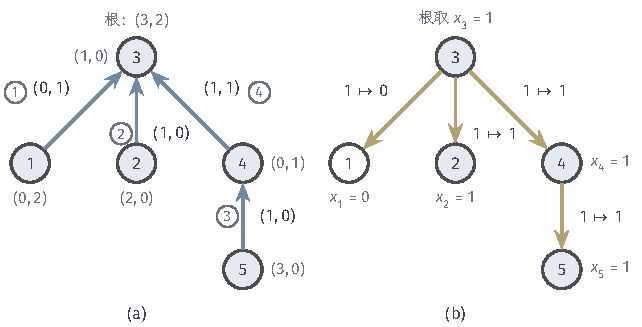
\includegraphics[width=108.514mm]{figures/01-basic-mathematics/04-graphs/tikz/c5-tree-messages/figure.pdf}
  \caption{分叉树上的消息与回溯。左：以$3$为根，按后序$1,2,5,4$发送消息；顶点旁的灰色二元组是一元项，箭头旁的二元组是消息表在接收端取$0$、$1$时的值，小圆圈中的序号是发送顺序；根合并后得到$(3,2)$。右：根取$x_3=1$后沿树向外查回溯表，黄色箭头旁的“$1\mapsto0$”表示父点取$1$时子点的最优选择为$0$；蓝色顶点取$1$，白色顶点取$0$，恢复的配置$(0,1,1,1,1)$成本为$2$。}
  \label{fig:graph-dp-tree-messages}
\end{figure}

把恢复的配置代回全部原始局部项，可以不依赖消息计算而独立核对结果。一元项依次为$0,0,0,1,0$，合计$1$；成对项中只有边$\{1,3\}$两端不同，贡献$1$；总成本为$2$，与根处的值一致，而且每个局部项只计了一次。

\subsubsection{算法分析}
\label{sec:graph-dp-tree-analysis}

\paragraph{正确性}
树上递推的正确性归结为一件事：每条消息确实是发送侧在接收端取值固定时的最低成本，即前面所说的报价单。

\begin{theorem}[树上消息的含义]
\label{thm:graph-dp-tree-message}
设依赖图$\mathcal G=(V,E)$是有限树，总成本由式~\eqref{eq:graph-dp-pairwise-cost}给出。对任意边$\{u,v\}$，记$F_{u|v}$为$u$一侧的部分成本：$V_{u|v}$中各顶点的一元项、两端都在$V_{u|v}$中的成对项，再加上边$\{u,v\}$上的$\phi_{u,v}$。则对每个$x_v$，
\[
m_{u\to v}(x_v)=\min_{\bm x_{V_{u|v}}}F_{u|v}(\bm x_{V_{u|v}},x_v).
\]
进一步，对任意根$\rho$，
\[
\min_{\bm x}F(\bm x)=\min_{x_\rho}\Bigl[\phi_\rho(x_\rho)+\sum_{r\in N(\rho)}m_{r\to\rho}(x_\rho)\Bigr].
\]
\end{theorem}

\begin{proof}
对$|V_{u|v}|$归纳。删去$u$以后，$V_{u|v}\setminus\{u\}$按$u$的其他邻居$r\in N(u)\setminus\{v\}$分成互不相交的部分$V_{r|u}$。由树中路径的唯一性，不同部分之间没有边，否则会与$u$形成环。因此$F_{u|v}$可以拆成
\[
F_{u|v}=\phi_u(x_u)+\phi_{u,v}(x_u,x_v)+\sum_{r\in N(u)\setminus\{v\}}F_{r|u},
\]
其中每个$F_{r|u}$只依赖$x_u$与$\bm x_{V_{r|u}}$，并且每个局部项恰好出现在其中一处。

固定$x_u$后，各$\bm x_{V_{r|u}}$是互不相交的变量组，由式~\eqref{eq:graph-dp-min-rules}后的第三条规则，对它们求最小值得到$\sum_r\min F_{r|u}$；由归纳假设，这个和等于$\sum_r m_{r\to u}(x_u)$。最后对$x_u$求最小值，就得到式~\eqref{eq:graph-dp-tree-message}。

叶顶点是归纳的起点，此时求和为空，结论直接由定义得出。根处的等式用同样的拆分得到：$V\setminus\{\rho\}$按$\rho$的邻居分成互不相交的部分，每部分的最小成本是一条入消息。
\end{proof}

链是树的特例：以$n$为根时$D_k(x_k)=\phi_k(x_k)+m_{k-1\to k}(x_k)$，定理再次给出$D_k$的含义。

回溯得到的配置也确实达到最优值。对子树大小归纳可知：若$x_v$已经确定，按回溯表给$u$一侧赋值后，$u$一侧的部分成本$F_{u|v}$恰好等于$m_{u\to v}(x_v)$，因为每一步选的$x_u$都达到式~\eqref{eq:graph-dp-tree-message}中的最小值，而子树内部又由归纳假设达到各条入消息的值。在根处合并后，总成本就等于根处的最小合并值。

这一论证要求根处最小值有限；为$+\infty$时任何配置都“达到”它，所以算法在这种情况下报告不可行，而不把回溯结果当作最优解输出。

回溯表只恢复一个最优配置。若要列出全部并列最优的配置，需要在每个状态记录全部最优选择，而这类配置的数目本身可能随$n$指数增长。

\paragraph{复杂度}
设每个变量至多有$q$个状态。处理非根顶点$u$时，汇总入消息需要对$x_u$的至多$q$个状态各加$|N(u)|-1$项，列候选与取最小共需至多$q^2$次加法和比较；对全部顶点求和，利用树中$\sum_u|N(u)|=2(n-1)$，向上一遍共需
\[
O\Bigl(\sum_u|N(u)|\,q+nq^2\Bigr)=O(nq^2)
\]
次运算。根处合并需要$O(|N(\rho)|q)$次，回溯只查$n-1$次表。存储为$n-1$张消息表和同样多的回溯表，每张至多$q$项。与$q^n$个配置的枚举相比，开销从指数降为线性于$n$，代价是要为每条边保存一张表。

\paragraph{适用范围}
本节的递推依赖两个条件。一是依赖图无环：定理的证明用到“删去$u$后各部分之间没有边”。二是局部项至多读取两个变量，使接口总是单个变量。依赖图含环时，删去一条边不再把变量分成两侧，单个变量不足以充当接口；下一节在四环上具体看这一点。

\subsubsection{各顶点的最小成本表}
\label{sec:graph-dp-tree-two-pass}

有时需要的不只是一个最优配置，而是每个顶点$v$取各状态$s$时整体能达到的最小成本$\min_{\bm x:\,x_v=s}F(\bm x)$，例如要知道某个变量换一个状态会多付多少。对根而言，这正是合并值$g_\rho$；对其他顶点，向上一遍只收集了来自子树一侧的消息，还缺父点一侧的报价。

所以再按前序从根向叶发送一遍消息，同样使用式~\eqref{eq:graph-dp-tree-message}：父点$v$向子点$u$发出的$m_{v\to u}$，汇总的是$v$的一元项、$v$的父点发来的消息和$v$的其他子点发来的消息。到达$u$时，$u$的全部邻居都已向它发过消息，把一元项与全部入消息相加，由定理~\ref{thm:graph-dp-tree-message}（以$u$为根）就得到$u$的最小成本表。两遍共发送$2(n-1)$条消息，开销仍为$O(nq^2)$。

图~\ref{fig:graph-tree-two-pass}只保留两遍发送的方向。第二遍仍然传递整张条件成本表；它与前面的回溯不同，回溯是在父点取值已经确定后读取一个达到者。

\begin{figure}[!htb]
  \centering
  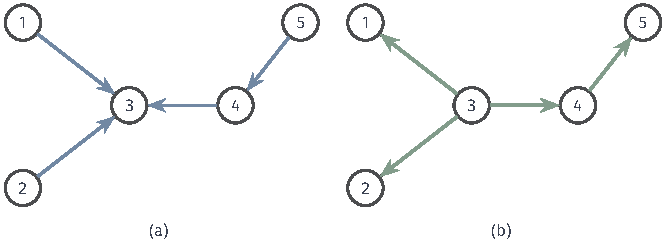
\includegraphics[width=107.500mm]{figures/03-graphs/04-local-functions-and-dynamic-programming/tikz/tree-two-pass/figure.pdf}
  \caption{两遍消息为每个顶点收齐各侧的信息。(a)以$3$为根，从叶向根传递蓝色消息；(b)按前序从根向外传递绿色消息，$3\to4$先于$4\to5$。两遍结束后每条无向边的两个方向都各发送一条表，共$2(n-1)$条；消息的索引是接收端的取值。}
  \label{fig:graph-tree-two-pass}
\end{figure}

在上例中，
\[
\begin{aligned}
m_{3\to1}(x_1)&=\min_{x_3}\bigl[\phi_3(x_3)+\phi_{1,3}(x_1,x_3)+m_{2\to3}(x_3)+m_{4\to3}(x_3)\bigr]\\
&=(2,1),
\end{aligned}
\]
其中$x_3=0,1$时一元项与两条入消息之和分别为$1+1+1=3$与$0+0+1=1$，再加上边$\{1,3\}$的成本取最小即得。于是$x_1$取$0$、$1$时的最小总成本为
\[
\phi_1+m_{3\to1}=(2,3).
\]

同样可得其余顶点的表：$x_2$为$(4,2)$，$x_3$为$(3,2)$，$x_4$为$(3,2)$，$x_5$为$(5,2)$。每张表的最小值都等于整体最优值$2$，并且都在最优配置$(0,1,1,1,1)$的相应分量处达到。

% 第11章第3节：从树到一般图（环带来的接口变化、四环算例、一般图动态规划的构建目标）。

\section{从树到一般图}
\label{sec:graph-dp-tree-to-general}

上一节的每一步都依赖一个事实：删去依赖树的一条边，变量就分成两侧，两侧只通过一个变量相连。依赖图含环时，这个事实不再成立。本节先说明环怎样改变接口，再用一个四环算例把变化落到具体数值上，最后说明一般图上的动态规划要事先构建什么。

\subsection{环带来的接口变化}
\label{sec:graph-dp-cycle-interface}

考虑四个变量排成的环$1-2-3-4-1$，每条边上有一个成对成本。删去边$\{1,2\}$后，剩下的是路径$2-3-4-1$，仍然连通：$x_1$不直接与$x_2$相连，却可以经由$x_4$和$x_3$影响$x_2$的最优选择。因此，沿一条边传递一张只以$x_2$为索引的报价单，无法概括$x_1$一侧，因为根本不存在只经过$x_2$与其余部分相连的“$x_1$一侧”。

链和树上的做法可以换一种说法，使它不依赖“一侧”。叶顶点$u$只出现在$\phi_u$和$\phi_{u,p(u)}$两项中；计算消息$m_{u\to p(u)}$，就是把这两项相加后对$x_u$取最小，然后用得到的表替换这两项。这个动作对任意局部函数集合都有意义。

设当前有一组函数，要汇总变量$x_i$。先找出当前全部作用域含$i$的函数，记为$\mathcal F_i$；它们的作用域之并去掉$i$，记为$S_i$。不含$i$的函数与$x_i$无关，可以留在最小化之外；含$i$的函数则必须一起处理。于是对$\bm x_{S_i}$的每种取值，把$\mathcal F_i$中的函数相加，再对$x_i$取最小，得到一个新函数
\begin{equation}
\psi_i(\bm x_{S_i})=\min_{x_i\in\mathcal X_i}\sum_{f\in\mathcal F_i}f .
\label{eq:graph-dp-elimination-step}
\end{equation}
然后从当前函数集合中删去$\mathcal F_i$，加入$\psi_i$；不含$i$的函数保持原样。这一操作称为消去$x_i$，按某个次序逐个消去变量的方法称为\term{变量消元}（variable elimination）。

消去$x_i$可以理解为替$x_i$提前做好决定。$x_i$的好坏只取决于$S_i$中那些与它同在某个函数里的变量；对这些变量的每一种取值，先算出$x_i$最好取什么、最少付多少，写成一张以$\bm x_{S_i}$为索引的表，此后其余变量只需查这张表，不必再关心$x_i$。由式~\eqref{eq:graph-dp-min-rules}的前两条，不含$i$的函数可以移出对$x_i$的最小化，所以替换前后，剩余变量每种取值下的最小成本不变；第~\ref{sec:graph-dp-min-cost-correctness}小节给出完整证明。

在树上消去叶顶点$u$时，$S_u=\{p(u)\}$，新函数就是消息$m_{u\to p(u)}$，接口仍是单个变量。在四环上消去$x_1$，情况不同：含$1$的函数是$\phi_{1,2}$与$\phi_{1,4}$，所以$S_1=\{2,4\}$，新函数$\psi_1(x_2,x_4)$同时读取$x_2$和$x_4$。在原来的环上，$2$与$4$并不相邻；消去$x_1$以后，它们通过$\psi_1$直接耦合在一起。

能否不要这张二元表，而给$2$和$4$各发一张单变量表？分别计算
\[
g(x_2)=\min_{x_1}\phi_{1,2}(x_1,x_2),\qquad h(x_4)=\min_{x_1}\phi_{1,4}(x_1,x_4)
\]
相当于允许两项各自为$x_1$挑选取值。由于每个$x_1$都满足$\phi_{1,2}+\phi_{1,4}\geq g(x_2)+h(x_4)$，对$x_1$取最小后总有
\[
g(x_2)+h(x_4)\leq\psi_1(x_2,x_4),
\]
但两边一般不相等：$x_1$只有一个，它在两项中必须取同一个值。下一小节的数值会说明，这个差异不仅是这一种拆法的缺陷，而且任何单变量表之和都无法代替$\psi_1$。

还有一种看似自然的做法，是在含环的依赖图上照搬式~\eqref{eq:graph-dp-tree-message}，让各顶点反复交换消息。这时同一部分成本会沿环被重复计入，上一节的正确性证明不再适用。这样的迭代是否收敛、收敛到什么，都需要另外分析；本部分只讨论精确计算。

\subsection{四环算例}
\label{sec:graph-dp-four-cycle}

本小节固定一个具体问题，后两章沿用它，分别演示两种结构构建和统一求值，避免更换例子掩盖它们之间的对应关系。四个二值变量$x_1,\ldots,x_4$排成环$1-2-3-4-1$，四条边上各有一个成对成本，没有一元项：
\begin{equation}
F(\bm x)=\phi_{1,2}(x_1,x_2)+\phi_{2,3}(x_2,x_3)+\phi_{3,4}(x_3,x_4)+\phi_{1,4}(x_1,x_4).
\label{eq:graph-dp-four-cycle}
\end{equation}
四张表由表~\ref{tab:graph-dp-four-cycle-costs}给出，每张表的行对应作用域中编号较小的变量。其中两个$+\infty$表示禁止的组合：$\phi_{3,4}(1,1)=+\infty$禁止$x_3,x_4$同时取$1$，$\phi_{1,4}(0,1)=+\infty$禁止$x_1=0$而$x_4=1$。

\begin{table}[!htb]
  \centering
  \begin{tabular}{cccc}
    \toprule
    $\phi_{1,2}(x_1,x_2)$ & $\phi_{2,3}(x_2,x_3)$ & $\phi_{3,4}(x_3,x_4)$ & $\phi_{1,4}(x_1,x_4)$\\
    \midrule
    $\begin{bmatrix}3&0\\1&2\end{bmatrix}$ &
    $\begin{bmatrix}1&3\\1&1\end{bmatrix}$ &
    $\begin{bmatrix}0&1\\0&+\infty\end{bmatrix}$ &
    $\begin{bmatrix}3&+\infty\\3&0\end{bmatrix}$\\
    \bottomrule
  \end{tabular}
  \caption{四环算例的局部成本。每张表的行对应作用域中编号较小的变量取$0,1$，列对应编号较大的变量取$0,1$；例如$\phi_{1,4}(0,1)=+\infty$。}
  \label{tab:graph-dp-four-cycle-costs}
\end{table}

\paragraph{枚举基准}
先用枚举给出核验基准。表~\ref{tab:graph-dp-four-cycle-enumeration}按字典序列出全部$16$个配置的总成本。其中$6$个配置被禁止：$x_4=1$而$x_1=0$的四个，以及$x_3=x_4=1$、$x_1=1$的两个。其余$10$个可行。

最小成本为$F^\star=3$，唯一的最优配置是$\bm x^\star=(1,0,0,1)$，此时四项依次为
\[
\phi_{1,2}(1,0)=1,\quad \phi_{2,3}(0,0)=1,\quad \phi_{3,4}(0,1)=1,\quad \phi_{1,4}(1,1)=0.
\]

\begin{table}[!htb]
  \centering
  \small
  \begin{tabular}{@{}cccccccc@{}}
    \toprule
    $0000$ & $0001$ & $0010$ & $0011$ & $0100$ & $0101$ & $0110$ & $0111$\\
    $7$ & $+\infty$ & $9$ & $+\infty$ & $4$ & $+\infty$ & $4$ & $+\infty$\\
    \midrule
    $1000$ & $1001$ & $1010$ & $1011$ & $1100$ & $1101$ & $1110$ & $1111$\\
    $5$ & $3$ & $7$ & $+\infty$ & $6$ & $4$ & $6$ & $+\infty$\\
    \bottomrule
  \end{tabular}
  \caption{四环算例全部配置的总成本。配置按$(x_1,x_2,x_3,x_4)$的字典序排列，前两行是$x_1=0$的八个配置，后两行是$x_1=1$的八个配置。}
  \label{tab:graph-dp-four-cycle-enumeration}
\end{table}

\paragraph{消去$x_1$}
按式~\eqref{eq:graph-dp-elimination-step}消去$x_1$。对$(x_2,x_4)$的每种取值，比较$x_1=0,1$两个候选$\phi_{1,2}(x_1,x_2)+\phi_{1,4}(x_1,x_4)$：
\[
\begin{aligned}
\psi_1(0,0)&=\min(3+3,\ 1+3)=4,&\qquad \psi_1(0,1)&=\min(3+\infty,\ 1+0)=1,\\
\psi_1(1,0)&=\min(0+3,\ 2+3)=3,&\qquad \psi_1(1,1)&=\min(0+\infty,\ 2+0)=2,
\end{aligned}
\]
达到最小值的$x_1$依次为$1,1,0,1$。

与之比较，分别取最小的单变量表是
\[
\begin{aligned}
g(x_2)&=\min_{x_1}\phi_{1,2}(x_1,x_2)=(1,0),\\
h(x_4)&=\min_{x_1}\phi_{1,4}(x_1,x_4)=(3,0).
\end{aligned}
\]
它们的和在$(x_2,x_4)=(1,1)$处为$0$，而$\psi_1(1,1)=2$：$g(1)=0$要求$x_1=0$，$h(1)=0$要求$x_1=1$，两项选的$x_1$互相矛盾。

更进一步，任何形如$g'(x_2)+h'(x_4)$的有限函数都满足
\[
\bigl[g'(0)+h'(0)\bigr]+\bigl[g'(1)+h'(1)\bigr]=\bigl[g'(0)+h'(1)\bigr]+\bigl[g'(1)+h'(0)\bigr],
\]
而$\psi_1$不满足这一等式：
\[
\psi_1(0,0)+\psi_1(1,1)=6\neq4=\psi_1(0,1)+\psi_1(1,0).
\]
所以$\psi_1$不能拆成两张单变量表之和，消去$x_1$以后的接口必须是$\{2,4\}$这两个变量的联合取值。

\paragraph{完成求值}
消去$x_1$后，剩下的函数是$\psi_1(x_2,x_4)$、$\phi_{2,3}(x_2,x_3)$与$\phi_{3,4}(x_3,x_4)$，只涉及$x_2,x_3,x_4$三个变量。把三项相加，按$(x_2,x_3,x_4)$的字典序得到
\[
(5,\ 3,\ 7,\ +\infty,\ 4,\ 4,\ 4,\ +\infty),
\]
最小值$3$在$(x_2,x_3,x_4)=(0,0,1)$处唯一达到。

再查$x_1$的选择：$(x_2,x_4)=(0,1)$时$x_1=1$。恢复的配置$(1,0,0,1)$与枚举结果一致。

这里同时处理的变量最多是三个：消去$x_1$时要看$\{1,2,4\}$的全部$8$种取值，最后又要看$\{2,3,4\}$的$8$种取值。第~\ref{chap:general-graph-dp-computation}章会把这一计算写成统一的递推，并用同一组数据检验最小成本、保留变量的成本表、计数和加权求和。

\subsection{一般图动态规划的构建目标}
\label{sec:graph-dp-construction-goal}

四环算例中的计算可以看成两个局部子问题。第一个子问题负责变量组$\{1,2,4\}$，固定接口$(x_2,x_4)$后汇总内部变量$x_1$，输出表$\psi_1$；第二个子问题负责$\{2,3,4\}$，读入$\psi_1$和其余两项，汇总全部剩余变量。链和树上的递推也是这样一族子问题，只是每个接口恰好是单个变量。

一般图上的动态规划要先构建这样一族子问题，它必须满足三项要求：
\begin{enumerate}
  \item 每个局部项都放进某个子问题，该子问题处理的变量包含它的整个作用域，并且每项只计一次；
  \item 摘要足够：一个子问题的内部变量与尚未处理部分的全部耦合都经过接口，所以以接口为索引的表不会丢失信息；
  \item 依赖可以排序：每个子问题只使用此前已完成的子问题的输出，最后汇总成整体结果。
\end{enumerate}
这三项都只涉及作用域和变量组，不涉及函数的具体数值，所以构建可以在求值之前单独完成。

树上递推正是满足这些要求的特例。把依赖树的一元项和成对项作为局部函数，按后序消去非根顶点：轮到$u$时，它的子点都已消去，子点留下的新函数与$\phi_u$、$\phi_{u,p(u)}$是仅有的含$u$的函数，所以$S_u=\{p(u)\}$，新函数$\psi_u$就是消息$m_{u\to p(u)}$，达到最小值的$x_u$就是回溯表$b_{u\to p(u)}$。

构建这族子问题有两种描述方式。变量消元用一个处理次序生成它们：每一步处理的变量组是当前变量及其$S_i$，新函数交给后面第一个用到它的步骤。树分解则把变量组（称为袋）和它们之间的接口显式组织成一棵树。第~\ref{chap:general-graph-dp-construction}章说明这两种构建怎样互相转换、怎样衡量其规模、怎样构造；第~\ref{chap:general-graph-dp-computation}章在构建好的结构上完成数值计算。四环算例已经显示，构建的质量体现为最多同时处理多少个变量，这里是三个。

\FloatBarrier
\section{本章小结}
\label{sec:tree-dp-chapter-summary}

本章的问题由局部函数组成：每个变量取有限个状态，整体成本是若干局部项之和，每一项只读取作用域中的少数变量，取值$+\infty$表示禁止的组合。同一份输入可以提出不同的输出要求：最小成本与一个最优配置、保留一组变量后的条件最小成本表、可行配置的个数，以及按局部权重之积定义的加权总和。枚举总能回答这些问题，但开销随变量数指数增长。

记录结构的几种图各有分工。原始图记录哪些变量共同出现，超图保留作用域的分组，因子图保留每个局部函数的身份；三者都不保存数值，原始图也不能恢复高阶规则，奇偶约束的例子说明三元规则不是成对规则的叠加。计算时始终使用完整的局部函数表。

链和树上之所以能精确递推，是因为删去依赖树的一条边就把变量分成两侧，两侧只通过一个接口变量相连。固定接口取值后，一侧的内部变量可以单独优化，结果写成以接口取值为索引的条件最小成本表；必须保留整张表，而不是一侧自己的最优值，因为接口最终取什么要等另一侧的成本也已知后才能决定。链上的递推、树上的消息和回溯表都是这一动作的具体形式，正确性来自有限集合上最小值的分步、移项和分离规则，开销对变量数是线性的。

依赖图含环时，单个变量不再能分隔两侧。消去一个变量会把它的邻居通过新函数耦合起来；四环算例中，消去$x_1$得到的$\psi_1(x_2,x_4)$不能拆成两张单变量表之和，接口必须同时保留两个变量。因此，一般图上的动态规划要先构建一族局部子问题，使每个局部项有处可放、接口足以概括内部变量、子问题的依赖可以排序；变量消元与树分解是描述这一构建的两种方式，分别在下一章建立并证明等价，数值计算统一放在第~\ref{chap:general-graph-dp-computation}章。

